
%%%%%%%%%%%%%%%%%%%%%%%%%%%%%%%%%%%%%%%%%%%%%%%%%%%%%%%%%%%%%%%%%%%%%%%%%%%%%%%%
\chapter{Apache Spark}
\label{sct:spark}
%%%%%%%%%%%%%%%%%%%%%%%%%%%%%%%%%%%%%%%%%%%%%%%%%%%%%%%%%%%%%%%%%%%%%%%%%%%%%%%%

Spark ist ein Programmierframework für Datenanalyse auf Clustern, was vor allemim Zusammenhang mit ''Big Data'' an Beliebtheit gewonnen hat.
Es vereinigt hierbei ausfallgehärtet Funktionalitäten von Batchverarbeitungssystemen bzw. Cluster-Management wie z.B. SLURM, Kommunikation zwischen Prozessen, wie z.B. OpenMPI und OpenMP sie zur Verfügung stellen, und zusätzliche problemspezifische Programmierbibliotheken.
Spark stellt Programmierschnittstellen für Java, Scala und Python zur Verfügung. Für Scala und Python existieren interaktive Eingabeaufforderungen mit der z.B. interaktive Echtzeitanalysen auf Clustern mit Spark möglich sind.\\

Apache Spark oder auch Spark Core stellt die Grundfunktionalität für verteiltes Rechnen bereit.
Das inkludiert die erwähnte Ausfallsicherheit, Management von Knoten über ein Web-Interface und Prozess-Scheduling\cite{learningspark}.
Die Programmierschnittstelle hierfür sind der Spark-Kontext und die Resilient Distributed Datasets (RDD).

\begin{figure}
    \centerline{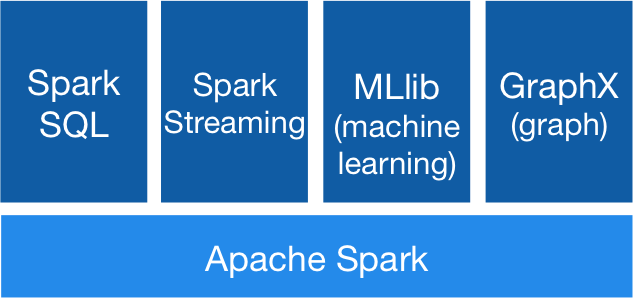
\includegraphics[width=0.5\linewidth]{spark-stack.png}}
    \caption{Zusammensetzung des Spark-Frameworks\cite{spark}}
    \label{fig:sparkstack}
\end{figure}

Beispielhaft für den Spark-Stack seien hier die Bibliotheken MLlib\cite{mllib} und GraphX erwähnt.

MLlib, kurz für Machine Learning Library, umfasst Funktionen wie lineare Regression, den K-Means-Algorithmus, Latent Dirichlet Allocation, Hauptkomponentenanalyse, das für Maschinenlernen benötigte stochastische Gradientenverfahren, u.v.m.

% GraphX
GraphX erweitert Spark-RDDs zu Kanten- und Knoten-RDDs die als Tupel einen Graph beschreiben \cite{graphx}. Auf diesen abgeleiteten Datentypen sind übliche RDD- und Mengenoperationen wie \lstinline!subgraph!, \lstinline!diff!, u.a. für das Erstellen und Modifizieren von Graphen möglich.
Ein solcher Graph kann z.B. Webseitenrelationen, jeder Link ist eine Kante im Graph, jede Domain ein Knoten, darstellen.
Auf diesen Graphen sind Algorithmen wie PageRank oder das Auszählen von Dreiecken in Graphen ausführbar.

%%%%%%%%%%%%%%%%%%%%%
\section{MapReduce}
%%%%%%%%%%%%%%%%%%%%%

Spark basiert auf dem MapReduce-Paradigma, welches 2004 in einem Paper der Google-Mitarbeiter Dean und Ghemawat\cite{mapreduce2004,mapreduce2008} in Anlehnung an die aus funktionalen Programmiersprachen bekannten Map- und Reduce-Befehle eingeführt wurden.
Viele der benötigten Algorithmen wie Häufigkeitsanalyse oder Webseitengraphen hatten zuvor ihren eigenen Programmcode für die Kommunikation und Ausfallsicherheit im Cluster und folgten von der Struktur her einem simplem Schema: zuerst werden Eingabedaten datenparallel verarbeitet und anschließend werden die Zwischenergebnisse zu Endergebnissen reduziert.
Diese einfach gestrickten Algorithmen mussten aber trotzdem auf beträchtlichen Datenmengen auf Knoten hoher Ausfallwahrscheinlichkeit laufen. Diese Funktionalität, also die Kommunikation im Cluster und die Ausfallsicherheit. wurde so in eine MapReduce-Bibliothek ausgelagert.

MapReduce bezeichnet hierbei sowohl das Programmierparadigma als auch die Bibliothek, die diese ausfallsicher und parallelisiert zur Verfügung stellt.
Dafür definiert der Nutzer eine Map-Funktion die aus einer Liste jedes Schlüssel-Wert-Paar $(k,v)$ auf eine Liste aus neuen Schlüssel-Wert-Paaren abbildet:
\begin{equation}
    \mathbf{Map : }\left( k, v \right) \mapsto
    \left[ \left( l_1, x_1 \right), \ldots, \left( l_{r_k}, x_{r_k} \right) \right]
\end{equation}
$k$ und $l$ sind hierbei die Schlüssel und $v$ und $x$ die dazugehörigen Werte. Für $r_k=1$ erhält man den Grenzfall, dass jeder Schlüssel-Wert-Tupel auf exakt einen neuen Schlüssel-Wert-Tupel abgebildet wird.

Da es per Definition keine Abhängigkeiten zu anderen Schlüssel-Wert-Paaren für die Berechnung der Map-Funktion gibt, kann jedes Datum parallel berechnet werden.
Das MapReduce-Framework stellt außerdem Funktionen zum Einlesen von Daten zur Verfügung und verteilt diese automatisch an die Knoten des Clusters, wo diese dann parallel verarbeitet werden.

In einem impliziten Schuffle-Schritt werden alle Paare mit gleichem Schlüssel lokal gruppiert, d.h. es werden alle Paare z.B. mit Schlüssel $k_1=\mathrm{'Dresden'}$ auf dem gleichen Knoten im Cluster gesammelt.
Dieser Schritt kann also sehr kommunikationsaufwendig sein.
Der Nutzer kann nur über die Art der Schlüssel auf diesen Prozess Einfluss nehmen.
Man erhält als Ergebnis des Schuffle-Schritts einen Tupel aus einem Schlüssel und einer Liste an dazugehörigen Werten.
\begin{equation}
    \mathbf{Shuffle :}
    \left[ \left( k_1, x_1 \right), \ldots, \left( k_n, x_n \right) \right]
    \mapsto \left[ \left( l_1, \left[ y^1_1, \ldots, y^1_{r_1} \right] \right), \ldots,
    \left( l_m, \left[ y^m_1, \ldots, y^m_{r_m}) \right] \right) \right]
\end{equation}

Im nachfolgenden Reduce Schritt werden die Tupel aus Schlüssel und Werteliste mit einer vom Nutzer defineirten Reduce-Funktion abgebildet auf eine neue Werteliste.
Im einfachsten Fall kann die neue Werteliste nur ein Element enthalten, z.B. die Summe oder den Mittelwert der alten Werte.
\begin{equation}
    \mathbf{Reduce : }
    \left( l, \left[ y_1, \ldots, y_{s_l} \right] \right)
    \mapsto \left[ w_1, \ldots, w_{m_l} \right]
\end{equation}

Auch die Reduce-Operation kann also bezüglich einzigartiger Schlüssel datenparallel ausgeführt werden.
Anfangs war dieses Paradigma nur für einfache Beispiele wie Wortfrequenzanalysen gedacht, aber mittlerweile wurden auch komplexere Algorithmen wie z.B. Matrixmultiplikation\cite{matmulmapreduce} oder das Problem des Finden einer maximalen Überdeckung\cite{maxcovermapreduce} ins MapReduce-Schema portiert.\\

%%%%%%%%%%%%%%%%%%%%%
% MapReduce
%%%%%%%%%%%%%%%%%%%%%

Eine lange Zeit beliebte Implementation basierend auf dem MapReduce-Paper\cite{mapreduce2004} ist Apache Hadoop\cite{hadoop}.
Hadoop besteht aus einem verteilten Dateisystem, dem Hadoop Distributed File System (HDFS), und einer Bibliothek namens MapReduce, die Funktionen für das Rechnen auf den verteilten Daten anbietet.

Apache Spark\cite{spark} ist eine alternative Implementation des MapReduce-Modells.
Es versucht viele der Probleme von Hadoop zu beheben, bietet jedoch neben dem Zugriff vom lokalen Dateisystem auch den Zugriff von HDFS und weiteren verteilten Dateisystemen aus an.

Einer der Hauptvorteile von Spark ist der Geschwindigkeitsgewinn bei der iterativen Anwendung von Map und Reduce durch die Möglichkeit die Daten auch im Arbeitsspeicher, nicht nur auf der Festplatte, der Knoten zwischenzuspeichern.


%%%%%%%%%%%%%%%%%%%%%%%%%%%%%%%%%%%%%%%%%%%%%%%%%%%%%%%%%%%%%%%%%%%%%%%%%%%%%%%%
\section{Architektur}
%%%%%%%%%%%%%%%%%%%%%%%%%%%%%%%%%%%%%%%%%%%%%%%%%%%%%%%%%%%%%%%%%%%%%%%%%%%%%%%%

% Executor, Masternode
Für kleinere Tests kann Spark local auf einem Computer bzw. Knoten ausgeführt werden:
\begin{lstlisting}[numbers=none]
spark-shell --master local[*]
\end{lstlisting}\vspace{-1.5\baselineskip}
In diesem Beispielaufruf der interaktiven Spark-Shell werden so viele Threads genutzt wie es logische Kerne gibt.

Für das Ausführen auf einem Cluster ist jedoch das getrennte Starten von einem Spark Driver (Master) und mindestens einem Executor (Slave, Worker) notwendig, vgl. \autoref{fig:sparkcluster}.
Der Spark-Driver führt das geschriebene Spark-Programm aus und verteilt u.a. die für die Map-Funktion benötigten Daten an die Executoren, welche die zugewiesenen Berechnungen dann durchführen.

\begin{figure}
    \centerline{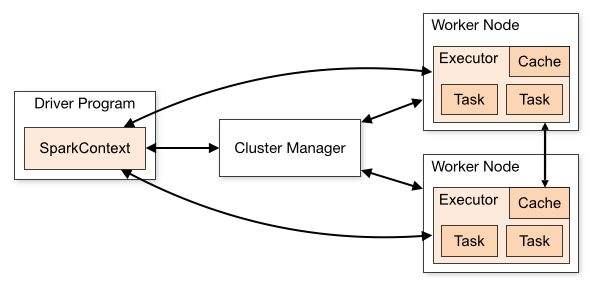
\includegraphics[width=0.8\linewidth]{cluster-overview.png}}
    \caption{Master/Slave-Struktur eines Spark-Clusters\cite{spark}}
    \label{fig:sparkcluster}
\end{figure}

Jeder Executor wird in einer eigenen Java Virtual Machine (JVM), also einem eigenen Prozess ausgeführt.
Normalerweise, und so auch hier, wird für jeden Knoten ein Executor-Prozess gestartet, welcher mit der in der \lstinline!SPARK_WORKER_CORES!-Umgebungsvariable definierten Anzahl an Threads arbeitet.
Für den hier vorgestellten Benchmark wird \lstinline!$SPARK_WORKER_CORES! identisch der Anzahl an Grafikkarten auf dem Knoten gewählt, sodass jeder Thread mit genau einer Grafikkarte arbeitet.\\

Ein RDD kann z.B. mit \lstinline!parallelize! erstellt werden \cite{sparkguide}.
\begin{lstlisting}[numbers=none,language=scala]
val distData = sc.parallelize( 1 to 10, 5 )
\end{lstlisting}\vspace{-1.5\baselineskip}
In diesem Beispiel wurden die Zahlen 1 bis 10 in ein RDD geladen.
Das zweite Argument gibt die Anzahl an Partitionen an, die das RDD nutzen soll.
Hier werden die Daten also in 5 Partitionen, in älteren Versionen von Spark auch Slices genannt, aufgeteilt.
Eine Partition ist wie ein Task zu verstehen, der von einem der Executoren ausgeführt wird.
Die Anzahl an Partitionen gibt damit eine Obergrenze für die Parallelisierbarkeit vor.
Um Gebrauch von einer optimalen Lastverteilung zu machen sollte man eine Größenordnung mehr Partitionen haben, als die Sparkinstanz logische Kerne bzw. Threads zur Verfügung hat.


%%%%%%%%%%%%%%%%%%%%%%%%%%%%%%%%%%%%%%%%%%%%%%%%%%%%%%%%%%%%%%%%%%%%%%%%%%%%%%%%
\section{Konfiguration von Spark auf einem Slurm-Cluster}
\label{sct:sparkconfig}
%%%%%%%%%%%%%%%%%%%%%%%%%%%%%%%%%%%%%%%%%%%%%%%%%%%%%%%%%%%%%%%%%%%%%%%%%%%%%%%%

Viele Cluster stellen schon einen Task-Scheduler für Multinutzerumgebungen, wie z.B. PBS (Portable Batch System) oder SLURM (Simple Linux Utility for Resource Management), zur Verfügung, um Rechenzeit auf dem Cluster möglichst effizient und gerecht zu verteilen.
Außerdem ermöglichen sie das verteilte Starten von Programmen, z.B. jene die mit MPI programmiert wurden.
Der für die Benchmarks genutzte Cluster, siehe \autoref{sct:taurus}, arbeitet mit SLURM.\\

Um Spark nutzen zu können, müssen zuerst Master- und Slave-Knoten gestartet werden.
Damit alle gleichzeitig gestartet werden, sollten sie innerhalb desselben Jobs initiiert werden.
Dies kann z.B. mit SLURMs \lstinline!--multi-prog! Option realisiert werden. Der Pfad zu der ausführbaren Datei wird dann als Konfigurationsdatei interpretiert, in der für jeden Rang ein möglicherweise anderes auszuführendes Programm angegeben ist. Beispielhaft:
\begin{lstlisting}[language=Bash]
> cat > test.conf <<EOF
0    echo master
1-3  echo slave
EOF
> srun -n 4 --multi-prog test.conf
0: master
2: slave
1: slave
3: slave
\end{lstlisting}\vspace{-1.5\baselineskip}

Alternativ kann man auch anhand von der Umgebungsvariable \lstinline!SLURM_PROCID! im Skript entweder einen Master-Knoten oder einen Slave-Knoten starten.
Diese Möglichkeit wurde aufgrund der Übersichtlichkeit, also weil damit alle Funktionalitäten in einem Skript vereint werden können, gewählt, siehe \lstinline!startSpark.sh!\attachfile{../startSpark.sh} und \lstinline!common/start_spark_slurm.sh!\attachfile{../common/start_spark_slurm.sh} \cite{scaromare}.

Auf dem Master-Knoten wird der Spark Driver mit
\begin{lstlisting}[language=Bash]
"$SPARK_ROOT/bin/spark-class" org.apache.spark.deploy.master.Master \
    --ip $(hostname) --port 7077 --webui-port 8080 &
\end{lstlisting}\vspace{-1.5\baselineskip}
gestartet.
Alle anderen Knoten starten einen Executor-Prozess mit:
\begin{lstlisting}[language=Bash]
"$SPARK_ROOT/bin/spark-class" org.apache.spark.deploy.worker.Worker \
    spark://$(scontrol show hostname $SLURM_NODELIST | head -n 1):7077
\end{lstlisting}\vspace{-1.5\baselineskip}
Hierbei wird vorausgesetzt, dass der Masterknoten, also jener für den \lstinline!$SLURM_PROCID=0! ist, der erste Knoten in \lstinline!$SLURM_NODELIST! ist. Dies wurde per assert vom Masterknoten aus auch geprüft und ist bei keinem der rund 50 Versuche fehlgeschlagen.

Wenn Spark gestartet ist, kann sich z.B. mit einer aktiven Eingabeaufforderung an den Master verbunden werden:
\begin{lstlisting}[language=bash]
export MASTER_ADDRESS=spark://$MASTER_IP:7077
spark-shell --master=$MASTER_ADDRESS
\end{lstlisting}\vspace{-1.5\baselineskip}
Die Umgebungsvariablen \lstinline!MASTER_ADDRESS! und \lstinline!MASTER_IP! werden automatisch von der Shellfunktion \lstinline!startSpark! gesetzt, siehe auch \autoref{sct:compilation}.
